\documentclass[11pt,a4paper]{article}
\usepackage[lmargin=1in,rmargin=1in,tmargin=1in,bmargin=1in]{geometry}
\usepackage[pagewise]{lineno} %line numbering
\usepackage{setspace}
\usepackage{ulem} %strikethrough - do not \sout{\cite{}}
\usepackage{xcolor} %change font color
\usepackage{graphicx}
\usepackage{filecontents}
\usepackage{tablefootnote}
\usepackage{footnotehyper}
%\usepackage{subfig}
\usepackage[yyyymmdd]{datetime} %date format
\renewcommand{\dateseparator}{.}
\graphicspath{{../img/}} %path to graphics
\setcounter{secnumdepth}{5} %set subsection to nth level
\usepackage{caption}
\captionsetup[table]{skip=11pt} %sets a space after table caption
\usepackage{times}
\usepackage{tabto} %general tabbed spacing
\usepackage{longtable} %need to put label at top under caption then \\ - use spacing
\usepackage[stable,hang,flushmargin]{footmisc} %footnotes in section titles and no indent
\usepackage[round]{natbib} %parenthesis instead of brackets for inline citations
\usepackage{enumitem}
\usepackage{boldline}
\usepackage{makecell}
\usepackage{booktabs}
\usepackage{amssymb}
\usepackage{amsmath}
\usepackage{physics}
\usepackage{tabularx}
\usepackage{multirow}
\usepackage{lscape}
\usepackage{array}
\usepackage{caption}
\usepackage{subcaption}
\usepackage[labelfont=bf]{caption}
\usepackage{chngcntr}
\usepackage{hyperref}

%\counterwithin{table}{section}

%\usepackage{xr}
%\externaldocument{} %aux file needed

\newcommand{\edit}[1]{\textcolor{blue}{#1}} %shortcut for changing font color on revised text
\newcommand{\fn}[1]{\footnote{#1}} %shortcut for footnote tag
\newcommand*\sq{\mathbin{\vcenter{\hbox{\rule{.3ex}{.3ex}}}}} %makes a small square as a separator $\sq$
\renewcommand\labelenumi{(\theenumi)} %changes 1. to (1) in enumerated list

\usepackage{fancyhdr}
\pagestyle{fancy}
\fancyhf{} %move page number to bottom right
\renewcommand{\headrulewidth}{0.5pt} %turn off line in header
\lhead{\scriptsize Prof. R. A. Borrelli} 
\chead{\scriptsize \textit{MCNP walkthrough - Part I}} 
\rhead{\scriptsize \today}
\rfoot{\thepage}

\begin{document}

\begin{titlepage}
    \title{
        \textbf{MCNP for Engineers}\\
        A walkthrough on how to use it, get results,\\
        and\\
        What it all means to a fulfilling life\\
        Part I - Super simple I promise!
    }
    \author{
        Prof. R. A. Borrelli
        \\ \\ \\
        University of Idaho $\sq$ Idaho Falls Center for Higher Education
        \\ \\
        Nuclear Engineering and Industrial Management Department
        \\ \\ \\
        rborrelli@uidaho.edu
        \\ \\ \\
        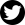
\includegraphics{twitter.png}
\includegraphics{git.png}\\
        @TheDoctorRAB\\ \\
    }
\clearpage %not have page number on title page
\maketitle
\thispagestyle{empty} %start with page number 1 on second page
\end{titlepage}

\chead{\scriptsize \textit{MCNP walkthrough - Preface}}

\section{Preface} \label{preface}
\subsection{Who is this walkthrough for?}
\noindent Advanced undergraduate students and graduate students in any nuclear engineering curriculum. Students should know - 
\begin{itemize}[leftmargin=*,topsep=0pt,itemsep=-1ex,partopsep=1ex,parsep=1ex]
    \item Basic nuclear physics; e.g., cross sections
    \item Interactions of neutrons and photons with matter
    \item Shielding, dose rates
    \item Four/six factor formula; e.g., what $k_{EFF}$ is,
    \item How a nuclear reactor works
    \item Solving for buckling
    \item Neutron diffusion
\end{itemize}
\vspace*{\baselineskip}

\noindent Just about every nuclear engineering department has this course. Typically, the Lamarsh or Duderstadt textbooks are used mostly. Sometimes the Shultis textbook is used. It's usually one of the first classes taken prior to the higher-level nuclear engineering courses. However, this course provides all you need to know to run and understand MCNP. I happen to teach this course. I use Lamarsh with Shultis as a reference. I happened to use Lamarsh because that was the textbook when I first took this kind of course. There really is no argument for one over the other.

\subsection{What is MCNP?}
\noindent Your best friend. Your greatest nemesis. MCNP is a contradiction. It will make you suffer, but it will open doors and present new opportunities. \\

\noindent MCNP is a computational tool - that means you're not coding \textit{per se}. You set up the input file that the code will read and then execute. MCNP tracks neutrons and photons for specified geometries and produces a wealth of resulting data. That seems simple. It's not. With a little guidance, effective modeling with MCNP is achievable. 

\subsection{Why is MCNP so important?}
\noindent It's not that necessarily MCNP itself is so important. Neutronics modeling is. We can't design any reactor without knowing where the neutrons are going and what they're going to do when they get there. MCNP happens to be the first neutronics computational tool. (They literally used punch cards.) All other tools are benchmarked against MCNP.\\

\noindent Not everyone is going to be a neutronics expert. For those that want to be, mastering MCNP makes it far easier to learn other neutronics codes, like Serpent. Any facility with MCNP provides a fundamental basis for a career in nuclear engineering. Frankly, if you're a graduate student, you're looking for internships. You may not really care what you're going to do; you just want a good position for your CV and a chance to network for future career development. Absolutely nothing wrong with that. On more than one occasion, I have had a researcher come up to me and ask `Do you know any of the students that know MCNP? I have some money for an intern this summer, but I need someone to step in and get right going.' I intend for this walkthrough to give you the skills to step right in and get going.\\

\noindent Learning MCNP will also lend to transferable skills. Whether it is good coding practices, geometric modeling, or just developing engineering judgement. This will lead to success in higher endeavors. \\

\newpage

\chead{\scriptsize \textit{MCNP walkthrough - Motivation}}

\section{Motivation - Do we \textit{really }need another `How to use MCNP'?} \label{motivation}
\subsection{Maybe?}
\noindent Don't read this if you don't want to. I'm not losing sleep over it. Due to the virus sweeping the nation in 2020, over the summer, I decided I needed to take the time to prepare my fall course with the contingency for shifting to online delivery. I've taught the course since 2015, so I know the material, have all the slides and assignments, etc., already prepared. This is part of that effort. Students should be able to follow this on their own and learn how to use MCNP. 

\subsection{An embarrassment of riches}
\noindent There are tons and tons and tons and tons of MCNP resources floating around out there. I have compiled them as I find them in my \href{https://courses.lumenlearning.com/uidaho-nuclear/}{online educational resource repository for nuclear engineering.} However, all this decentralization just spreads the materials out so much that there isn't really an orderly way to work through them as a learning process. There are a lot of good problems out there that I use in class. \\

\noindent Probably the closest resource to what I'm trying to do here is the famous \href{https://www.mne.k-state.edu/~jks/MCNPprmr.pdf}{MCNP primer} from Prof. Shultis at Kansas State University. A particularly good feature of the primer is that it cross references to the MCNP manual. I certainly used it when I first learned MCNP. However, I do not know if that manual is shipped with MCNP anymore, and the most recent revision of the primer that I have found is 2011. To be fair, not too much has changed in the ensuing time, but just about all of the resources in addition to the primer that I have found are somewhat dated. The time seems right to develop something new. Another difficulty I have is that most of these resources are gigantic information dumps. It was overwhelming for me when I was first learning MCNP. I like writing, I'm fairly good at it, and given the context of 2020, the time felt right to give this a shot. \\

\newpage

\chead{\scriptsize \textit{MCNP walkthrough - Personal}}

\section{Experience - And who do you think you are?} \label{experience}
\noindent Well, I'm an actual nuclear engineering professor. I've taught the Lamarsh class with an MCNP learning module every year since 2015. Students have attained solid success with publications, internships, and gainful employment from the course. I have many publications applying MCNP in a variety of topics. My expertise in MCNP has led to several funded projects. Ask about me. \\

\noindent I am by no means the leading expert in MCNP. I'm probably not a leading anything unless I'm leading you to happy hour. I can name probably 12 - 15 people I know personally that are better at neutronics modeling than me, and probably 3 to 5 of them are students that took my course. However, actually \textit{teaching} MCNP formally is a different paradigm, altogether. I am confident that I'm on a short list of being able to teach \textit{how to use MCNP effectively}. I am purposely very specific in claiming what I can actually do here.

\section{Style - What's wrong with you?}
\noindent Plenty, but now's not that time for that. \\

\noindent As you may have gathered so far, my tone is intended to be conversational and not overly ponderous. So, not like a journal paper. I'm writing in the way I have been lecturing on MCNP. I'm trying to ease you through the learning process and not just dump everything on to the page. I'm not trying to talk down to anyone. I know the difficulties I had with learning MCNP, so I'm writing in a way that I would have wanted to be spoken to. Even that's a bad sentence, but this isn't meant to be a formally reviewed and published document.\\

\newpage

\chead{\scriptsize \textit{MCNP walkthrough - Intent and direction}}

\section{Teaching MCNP for \textit{engineers}}
\noindent There is a reason why I chose the title that I did. I'm interested in getting students and other researchers the guidance they need to run MCNP. If I were going to prepare a course, then, sure, I would spend a significant time on Monte Carlo theory. And I'll have a brief section in here about that. I'm not arguing that a scientific approach isn't valuable in comparison to an engineering approach. I have found most MCNP resources include a ton of material on the theory behind MCNP. I'm assuming you know that already. If you feel like you need some background on the theory behind MCNP, I direct you to \href{https://laws.lanl.gov/vhosts/mcnp.lanl.gov/pdf_files/la-ur-05-4983.pdf}{Fundamentals of Monte Carlo particle transport} by Dr. Forrest B. Brown at Los Alamos National Laboratory. If there's only one expert in MCNP and Monte Carlo theory, he is probably that person. 

\section{\textit{Walkthrough}}
\noindent I also chose the term `\textit{walkthrough}' deliberately. Here's where I think I bring some value versus other resources. When I think about a walkthrough, I'm thinking about video games - You're playing a cool game but for the last hour you're stuck in a room looking for a lever or loose tile or you're asking questions to the townspeople and you know you have to do it in a certain order but you're going in circles. The game is starting to get tedious and you need a hint. The walkthrough provides a detailed account of the game - right down to where to look or, not only what weapon to select, but what move to employ. That's what I'm going for here - `Fatal error? Look up. Unlatch the window.' MCNP is slightly more complex than a video game, but if you can build an input file from scratch and get it to run, then you're well on your way. Building in more complexity isn't as overwhelming. 

\newpage

\chead{\scriptsize \textit{MCNP walkthrough - Getting started}}

\section{Installation}
\noindent Detailed installation instructions are provided with your MCNP disks. I am not going to repeat them here, but you should follow them to the letter. Run the tests after to make sure everything is all set. Remember, your license only allows you to install MCNP in one place due to export control restrictions. Mine is on my office desktop. I do not recommend installing it on a laptop. If it gets stolen, you could get into some trouble. Your license is granted through your institution. If you change positions and go somewhere else, then you need to apply for another license and you have to uninstall the distribution under the prior license and destroy the disks. 

\section{Operating system}
\noindent I strongly recommend installing in linux. Over the years, I've experienced either first hand or with students, inexplicable wonkiness with MCNP in a Windows environment. Don't have a linux system? No problem! You can install a `virtual linux machine' on your windows computer. It takes some time, but it's not hard. I have MCNP installed on the virtual machine in my office. I am using the `Oracle VM VirtualBox Manager'. That is basically the holder for your linux environment. I use the CentOS8 linux system. There's others to choose from. If you have the computing power, you can have the box make two screens or more if you have a multiple monitors. I actually use the linux box about 99\% of the time for MCNP, data processing, lecture slides, presentations, papers, all of it. 

\section{Visualization}
\noindent The linux distribution for MCNP comes with a plotter equipped to view your models. There's nothing extra to do in a standard linux environment. MCNP used to ship VisEd. I started on VisEd, so I am more used to it than the plotter. Both aren't super great. VisEd only runs in windows. You can request a VisEd download separately after you obtain your MCNP license. I would recommend it. Try both. It's kind of a pain to copy your MCNP file from linux to windows, but it's not really that bad.

\section{Manual}
\noindent The MCNP manual is very comprehensive. That's also kind of the problem. When I was learning MCNP on my own, the manual was just overwhemling. It is important to have even if for showing what each card (essentially, a card is a command) default is, or what output you want to write. Additionally, it contains several tables for the cross section libraries that you can designate. The `standard' manual which I think everyone refers to when they're talking about the manual is the one with the \textit{LA-UR-03-1987} designation. Mine was last revised in 2008. I don't know if this is shipped or not with the most current MCNP distribution, but I would recommend to find it. I'm not going to be referring to the manual. The Primer actually does a good job with that. I'm intending this walkthrough to be standalone, where the user can then access more comprehensive resources and not feel deluged with information.

\section{Text editor}
\noindent MCNP is a FORTRAN code. \textit{FORTRAN}. That's an old language. O. L. D. That means you have to be really careful in your selection of a text editor. FORTRAN will go sideways fast if there's any whitespace or `$\wedge M$' in there. It is also very column specific - where to start and end a line. This is because when they first invented the language, they were programming on punch cards. Fortunately, there are plenty of choices in linux that can be used to build your input files. I use \texttt{vim}. I started on \texttt{vi} at an internship in undergrad at the Naval Undersea Warfare Center because the particular group I was working in used that. I actually learned FORTRAN there. The other popular editor is \texttt{emacs}. In linux, there are many choices. Use one of these. Make sure to turn on line numbers!

\section{Scientific computing best practices}
\subsection{Python}
\noindent As a nuclear engineering graduate student, faculty, or other professional, I know you all have a copy of \href{https://www.google.com/books/edition/Effective_Computation_in_Physics/6IkNCgAAQBAJ?hl=en&gbpv=0}{Effective Computation in Physics: Field Guide to Research with Python}. This book, and I feel like using the term `book' to describe this treatise to a successful research career just falls short, should be your guide to best computing practices. Again, installing MCNP in linux allows for more ready postprocessing with the accessibility to python. You can install python in your windows environment, but I just find installing packages to be a lot easier in linux. 

\subsection{Postprocessing}
\noindent For more complex neutronics and/or photon modeling, effective postprocessing is a necessity. Fortunately, with python, you can find many scripts to edit for your own purposes. I have several on my github. Please feel free to look around my repositories. Additionally, I've found it easier to prepare graphs in python. I have several python graph scripts as well. MCNP comes with plotting capabilities. I never got around to learning how to use them yet. That doesn't mean they aren't
useful. I just haven't had the time. You can also explore the \href{https://pyne.io/}{PyNE toolkit}.

\subsection{Reproducibility}
\noindent Good computing means your creation can be used by other people. If you make an MCNP file, someone else should be able to run it and produce the same results that you obtained. This provides confidence that you produced research that is scientifically sound. Then, whomever has your MCNP file can modify, enhance, or build upon the model to tackle more problems. We must have this principle in mind when developing MCNP files. Much of that just involves comprehensive commenting. As I walkthrough MCNP, I'll make note of this. 

\newpage

\chead{\scriptsize \textit{MCNP walkthrough - Theory}}

\section{A brief discussion on Monte Carlo theory}
\noindent The theory behind MCNP is fairly complicated. It would take a semester course to really get into it in depth. I don't really teach much of it at all, just enough so a user knows how MCNP works. Dr. Brown's 400+ slides contain an exhaustive amount of information on Monte Carlo theory, and I have used them for my own lectures in the Lamarsh course. I'm not trying to be glib - it's important to know the theory. However, this is a walkthrough for engineers on how to use MCNP. The theory can be discovered elsewhere.\\

\noindent In short - Monte Carlo in general is a mathematical approach that simulates particle transport using lots of random number generators and statistical distributions. I'm sure the savvy graduate student will quickly understand that the science of random numbers is of critical importance. True randomness can't ever be achieved, but you need your simulation to be as high fidelity as possible. Dr. Brown's slides contain a very in-depth discussion about random number generation in MCNP. It's
very good. Both the slides and the generation of randomness. I'm not a benchmark expert, but I think this is one of the reasons everything is benchmarked with MCNP. The user can actually change the kernels for random number generation, but I have never done that. 

\subsection{MCNP solves the transport equation}
\noindent Monte Carlo methods solve integral problems, and it is very applicable to multi-dimensional integration. This is great for us because we're concerned with where the neutrons are born, where they're going, and what happens when they get there. Lots and lots and lots of times over. \\

\noindent For completeness, the Boltzmann transport equation is - 
\begin{equation} \label{eq-transport}
    \Psi(\underline{r},\underline{v})=\int[\int\Psi(\underline{r}',\underline{v}')C(\underline{v}'\rightarrow\underline{v})d\underline{v}'+Q(\underline{r}',\underline{v})]T(\underline{r}'\rightarrow\underline{r})d\underline{r}'
\end{equation}

\noindent Where - \\
\begin{enumerate}[topsep=0pt,itemsep=-1ex,partopsep=1ex,parsep=1ex]
    \item[]$\Psi(\underline{r},\underline{v})$ - particle collision density
    \item[]$Q(\underline{r}',\underline{v})$ - source density; fixed, fission, eigenvalue
    \item[]$C(\underline{v}'\rightarrow\underline{v})$ - collision density; velocity change at fixed position
    \item[]$T(\underline{r}'\rightarrow\underline{r})$ - transport density; position change at a fixed velocity
\end{enumerate}
\vspace*{\baselineskip}

\noindent Monte Carlo methods will then employ a Markov scheme applying superposition to solve the integral equation. The trick is that the use of Markov makes the solution `memoryless'; the current state of the particle is only dependent on the prior state. Then, \textit{histories} are simulated for a particle, or a sequence of states. Each occurence in the sequence is then \textit{tallied}. These terms are frequently used in MCNP so I wanted to define them here. \\

\noindent MCNP then simulates a single particle history from birth to death by tallying the random walk for the particle. Collisions are modeled by physics equations and cross sections. The free flight of the particle is modeled using the computational geometry of the model. \\

\noindent There are a few assumptions that are inherent in Monte Carlo solutions. 
\begin{enumerate}[topsep=0pt,itemsep=-1ex,partopsep=1ex,parsep=1ex]
    \item The medium is static and homogeneous. Although use of homogeneous here just means it doesn't change. 
    \item The solution is time independent. 
    \item Markov principles are appled. 
    \item Relativistic effects are neglected.
    \item Particle `fly' in straight lines. 
\end{enumerate}
\vspace*{\baselineskip}

\noindent Right off the bat, you can see that for reactor concepts like a molten salt reactor, MCNP isn't the best choice, althought it will produce reasonably meaningful results. However, MCNP can solve a wide variety of problems. Even if using newer Monte Carlo computational tools, I would still recommend learning MCNP first.  

\subsection{Using Monte Carlo to compute $\pi$}
\noindent Computation of $\pi$ by Monte Carlo methods is a classic and fun example to illustrate the theory.\\

\noindent We know $\pi$ has a special relationship with a circle. 

\begin{figure}[h!]
    \centering
    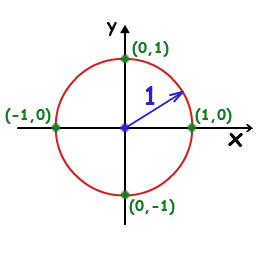
\includegraphics[width=0.25\textwidth]{circle.png}
    \caption{A unit circle.}
    \label{fig-circle}
\end{figure}

\noindent The equation of the circle is - 
\begin{equation} \label{eq-circle}
    x^2 + y^2 = 1
\end{equation}

\noindent And the area of this circle is - 
\begin{equation} \label{eq-area}
    A = \pi r^2 = \pi (1^2) = \pi
\end{equation}

\noindent The procedure is then - 
\begin{enumerate}[topsep=0pt,itemsep=-1ex,partopsep=1ex,parsep=1ex]
    \item Sample a random number for $x \in (0,1)$.
    \item Sample a random number for $y \in (0,1)$.
    \item Input $x,y$ into Equation \ref{eq-circle}.
    \item Compute Equation \ref{eq-circle}.
    \item If the result is greater than 1, then discard.
    \item If the result is less than 1, then record. (I call it a `hit'.)
    \item Repeat for N times. 
    \item Tally the total number of hits. 
    \item Divide the total hits by N.
\end{enumerate}
\vspace*{\baselineskip}

\noindent Looking a Figure \ref{fig-circle}, you'll see we're recording the hits to the first quadrant of the circle. Essentially, we've evaluated the integral - 
\begin{equation}
    G = \int_0^1 \sqrt{1-x^2} dx = \frac{1}{2}(x\sqrt{1-x^2} - sin^{-1}x)|_{0,1} = \frac{\pi}{4}
\end{equation}

\noindent To get $\pi$, multiply the result by 4.\\

\noindent Each `particle' that is generated; i.e., $(x,y)$ pair, is independent on the prior particle. Here, the `interaction' is only whether the particle falls within the boundary. With a neutron, this could be a scattering or absorption event, which would be determined by cross sections and probability density functions. The concept is essentially the same on a fundamental level. \\

\noindent It should be clear that the choice of N is important. Increasing N will result in solution convergence. I have a \href{https://github.com/TheDoctorRAB/education/blob/master/src/monte.carlo.simple.py}{python routine} where you can experiment with the selection of N and observe the convergence. In fact, that's typically the first option in MCNP when the statistics aren't working out - increase the number of particles to generate more histories. \\

\noindent That's the extent of theory that is really necessary to run MCNP. Of course, as higher level problems pop up, you'll need to learn more, but this discussion should give you enough of a base that you'll be able to understand the theory in more depth if needed. And that's really engineering in a nutshell - learn what you need to solve the problem and whatever else comes after. 

\newpage

\chead{\scriptsize \textit{MCNP walkthrough - Getting to know Jezebel}}

\section{Getting to know the MCNP input file}
\noindent Jezebel is the most basic MCNP problem. Everyone knows it. It is a bare Pu sphere with a Ni reflector. We'll start with a model of just a bare Pu sphere. We want to find the critical size. Download the \href{https://github.com/TheDoctorRAB/mcnpx.decks/blob/master/criticality/jezebel-light.inp}{input file} and open it in your text editor. I'll be referring to line numbers, so turn that on. \\

\noindent The next page has a copy of the input file. 

\newpage

\subsection{MCNP input file for a bare Pu sphere}

\begin{tiny}
\begin{verbatim}
Jezebel bare Pu sphere
c      -----------------------------------------------------------------
c      R.A.Borrelli
c      -----------------------------------------------------------------
c      rev.22.August.2014
c      -----------------------------------------------------------------
c
c      ------------------------- MODEL NOTES ---------------------------
c
c      The origin is the center of the sphere.
c      
c      ----------------------- END MODEL NOTES -------------------------
c
c      -----------------------------------------------------------------
c
c      ------------------------- START CARDS ---------------------------
c
c      -----------
c      cell cards
c      -----------
c
c      ---
100    1 -19.86       -10       imp:n=1       $plutonium sphere
c      ---
c
c      ---
150    0               11       imp:n=0       $void
c      ---
c
c      -----------
c      end cell cards
c      -----------

c      -----------
c      surface cards
c      -----------
c
c      ---
c      geometry
c      ---
10     SPH  6.38493     $plutonium sphere
c      ---
c      end geometry
c      ---
c
c      -----------
c      end surface cards
c      -----------

c      -----------
c      physics cards
c      -----------
c
c      ---
MODE   n
c      ---
c
c      ---
c      end physics cards
c      ---
c
c      ---
c      source
c      ---
c
c      ---
KCODE  1000 1.0 30 130
KSRC   0 0 0
c      ---
c
c      ---
c      end source
c      ---
c
c      ---
c      materials
c      ---
c
c      ---
c      plutonium
M1     94239.66c 1.0
c      ---
c
c      ---
c      end materials
c      ---
c
c      ----------- END CARDS -----------
c
c      -----------------------------------------------------------------
\end{verbatim}
\end{tiny}

\newpage

\subsection{General MCNP input file format}
\subsubsection{Title card}
\noindent The very first line of the file is the title card. MCNP will print the title to the output file. This may be a relic of an old age because you can name the output file when you run MCNP on the command line. I suppose back when you had physical cards, this wasn't the case. 

\subsubsection{Comments}
\noindent The MCNP input file is separated into `cards'. I will talk about the format of the MCNP in general and then each card. First of all, note that \texttt{c} designates a commented line; i.e., the code won't read it. I know everyone probably knows this, but I'm being tedious on purpose to walk you through the code. Obviously, anything not commented out is read by the code. In addition to the \texttt{c} for commented lines, there is the use of \texttt{\$} as a comment where a line is a card. In line 23, the cell labeled \texttt{100} ends with \texttt{\$plutonium sphere}. Obviously, this means that the cell is the sphere of plutionium for which we are modeling for critical size. \\

\noindent Even for this simple model, you'll see my input file (also called as deck - as in deck of cards) is extensively commented. This is just good coding practice. Anyone not even remotely familiar with MCNP can see in the file what goes where. This is an older file, so I have my name and the date. I made this file before I had github. If you're using github, it's probably not necessary to include the date. I'd also put my github/twitter handle instead of my full name because it's easier to
find me that way. A more recent deck for my \href{https://github.com/TheDoctorRAB/igem/blob/master/neutronics-shielding/low-burnup/L-3030/guide-assembly/container/air/borosilicate-glass-backfill/10cm/0wt/10wt/12cm/inp/single.assembly_7815.inp}{used fuel cask} is more extensively commented. \\

\noindent I have model notes section to describe what the geometry is, etc. I would strongly recommend to note the origin in the geometry, especially when the geometry becomes increasingly complicated. Here, the origin is the center of the Pu sphere. MCNP doesn't actually care where the origin is because you actually define the geometry relative to the origin. Noting the origin in the comments is helpful in case you forget, or if someone else is going to use the file. \\

\noindent Next, I have a \texttt{START CARDS} comment. This is just so I know where the actual MCNP starts. It helps when the model notes section is extensive because I can just search the keyword in \texttt{vim} and go right to the start. \\

\noindent The dollar sign `\$' is used as an inline comment. Don't use it in column 1. On line 23, there is a comment indicating that this line describes the plutonium sphere. 

\noindent MCNP contains cell, surface, physics, source, materials, and print cards. These are all indicated in the file comments, except the print cards. We'll do that later when we add the reflector. 

\subsubsection{Blank lines}
\noindent There are only TWO blank lines in the file. Line 34 and line 50. That's it. You will get the dreaded FATAL ERROR if there are more or if they are in the wrong position. One is at the end of the cell cards, and the other at the end of the surface cards. At lines 51,52 where I indicated the physics cards, to the end of the file is collectively called the data cards. I divided it up so I can just search by keyword. \\

\subsubsection{FORTRAN format}
\noindent Excluding the comments, there are some `commands' that start in column 1. Each of these can be considered a card, specific to the section it is in. On line 82, a material card is designated \texttt{M1}. It is for the plutonium. I include a comment that labels the material. What would \texttt{100} mean? You can see it is in the cell card section, so it is a card designating cell 100. \\

\noindent I use capitals for the card designations. It's not necessary. When the file gets really large though, it's just easier to read. \\

\noindent After each card, there is more information that defines the card. Note that the card information always starts in column 8. This is because of FORTRAN. Similarly, FORTRAN is limited to 80 columns per line. 

\subsection{Detailed card descriptions}
\subsubsection{Cell cards}
\noindent Cell cards come first in the file. But what exactly is cell? A cell is an object you want to model or part of the geometry environment. A room could be a cell, but you might want to model the dose rate of material in the room. A cell can be a collection of cells. A fuel rod is a cell. However, the rod is composed of pins, which are also cells. \\

\noindent Cells are defined by an assemblage of surfaces that you define in the surface card section.\\

\noindent For my first cell card, I designate the cell that can't be further decomposed into other cells. There's no required way to list the cell cards, but I recommend to pick a style and stick with it. \\

\noindent I label cells starting with \texttt{100}. This is just a style convention. Cell, surface, and material cards can have the same label, but you can see that this could be confusing for complicated geometries. \\

\noindent In this example, the first cell is the plutonium sphere. After the cell designation (\texttt{100}), the next piece of information is a \texttt{1}. This refers to material 1, which is plutonium. Next, there is a \texttt{-19.86}. This is the material density. Use of the negative sign indicates that the density is given in grams per cubic centimeter. Use of a positive number would indicate units of atom density. A $+$ sign is not used. I like to stick to mass density because it's easy to look up
quickly. \href{https://www.pnnl.gov/main/publications/external/technical_reports/PNNL-15870Rev1.pdf}{PNNL} has compiled a document of over 350 materials with densities and atom fractions for over 350 materials. \\

\noindent The next piece of information is a \texttt{-10}. This is the surface card that comprises the cell. Here, we only have one surface, which is the sphere. For a room, there would be six surfaces. The negative sign indicates the `sense' of the surface, and this will be discussed separately. \\

\noindent Finally, there is \texttt{imp:n=1}. This denotes the cell importance for neutrons. Just about all MCNP problems will have a cell importance of 1. This just means that a neutron entering or born in the cell will be treated as one neutron when MCNP `tracks' it. Each cell must have an importance. \\

\noindent I've changed the cell importance a grand total of one time in my decades of using MCNP. Leave it as 1. \\

\noindent A second cell is also listed (\texttt{150}). What is different about it when compared to cell \texttt{100}? Because I commented the file well, it is clear that this is void cell. In MCNP, the last cell always has to be a void. It is literally the nothingness that exists outside the model universe. Who knew MCNP was so zen? The material will always be \texttt{0}, and the neutron importance is zero \texttt{imp:n=0}. A neutron entering the void just disappears and is not
tracked. \\

\noindent How does MCNP know exactly what is the void? This comes back to sense. The void is essentially the complemenatary sense of all the outer cell boundaries to it. This is fairly easy here because the void is just the positive sense to surface 10, which is just the Pu sphere. This will become clearer when we discuss sense. \\

\noindent As a final note, the spacing of each piece if information is not relevant. I like to have everything line up. For teaching, it's just easier for the class to see the information on the card when it's displayed up on the sceen. The order is important. And the material designation must start in column 8.

\noindent\textbf{Review.}\\
\noindent\texttt{100    1 -19.86       -10       imp:n=1       \$plutonium sphere}\\

\begin{enumerate}[topsep=0pt,itemsep=-1ex,partopsep=1ex,parsep=1ex]
    \item cell label - \texttt{100}
    \item material definition - \texttt{1}
    \item mass density - \texttt{-19.86}
    \item surface definitions and sense - \texttt{-10}
    \item importance - \texttt{imp:n=1}
    \item comment
\end{enumerate}
\vspace*{\baselineskip}

\noindent It doesn't matter how complicated the geometry gets. The cell cards all have the same format!

\subsubsection{Surface cards}
\noindent After the cell cards is a \textbf{BLANK LINE}. \\

\noindent Then, the surface cards are defined.\\

\noindent For this problem, the only surface is the Pu sphere. On line 42, similar with the cell cards, it starts with the surface label, \texttt{10}. Again, there isn't any numbering convention. I like to use double digit numbers for the label. I also commented that this surface defined the fission source. \\

\noindent Next, \texttt{SPH} defines the surface, a sphere. Of course, there are numerous surface definitions. These are in the manual. I'm not going to dump them all out here. \\

\noindent When defining any surface, numerical dimensions are required. For \texttt{SPH} only requires a radius - \texttt{6.38493}. That's it! Capitals aren't needed. It is just my style convention. 

\noindent Looking at cell \texttt{100}, you can now see that the cell is comprised of surface \texttt{10} with negative sense. In this case, the cell is the single surface with the defined sense and importance.

\noindent\textbf{Review.}\\
\noindent\texttt{10     SPH  6.38493     \$plutonium sphere}\\

\begin{enumerate}[topsep=0pt,itemsep=-1ex,partopsep=1ex,parsep=1ex]
    \item surface label - \texttt{10}
    \item surface definition - \texttt{SPH}
    \item surface dimensions - \texttt{6.38493}
    \item comment
\end{enumerate}

\subsubsection{Physics cards}
\noindent MCNP allows the user to define all sorts of physics models. I rarely have used any for the problems I've worked on. In this file, I have included \texttt{MODE   n} to designate neutron transport. This is the default so it is not really needed. I include it for completeness. You can add \texttt{MODE   n p e} for photons and electrons, respecively. So, I have the card in place already in case I need to include photons or electrons. Since we are only interested in determining
the critical mass for the bare Pu sphere, the neutrons are all we care about. It doesn't hurt to be overly deliberate
though.

\subsubsection{Source cards}
\noindent MCNP requires a source to be defined. For computations involving $k_{EFF}$, the \texttt{KCODE} and \texttt{KSRC}. The \texttt{SDEF} card can be used in place of the \texttt{KSRC} card for more complicated problems. It actually offers an enormous amount of flexiblity. That is a topic for a higher level walkthrough. \\

\noindent The \texttt{KSRC} card contains x y z coordinates designating a fission source point. Essentially, where each neutron is first `born'. It stands to reason then that you want to make sure you designate the source point within the cell containing the fissile material. This is another reason why it's important to note where the origin is. Here, a source point is designated at the orgin - \texttt{0 0 0}. From experience, I know this is sufficient. However, I could have as many as
I want. If we had two spheres, source points should be designated in each. \\

\noindent The \texttt{KCODE} card tells MCNP to compute $k_{EFF}$ and how to do it. 

\end{document}
